\pdfoutput=1
\documentclass{article}

\usepackage{arxiv}
\usepackage[utf8]{inputenc}
\usepackage[T1]{fontenc}
\usepackage{hyperref}
\usepackage{url}
\usepackage{booktabs}
\usepackage{amsmath,amssymb,amsfonts,amsthm}
\theoremstyle{definition}
\newtheorem{definition}{Definition}
\newtheorem{corollary}{Corollary}
\usepackage{graphicx}
\usepackage{xcolor}
\usepackage{tikz}
\usetikzlibrary{arrows.meta,positioning,fit,calc}
\usepackage[numbers,sort&compress]{natbib}
\usepackage{microtype}
\usepackage{algorithm}
\usepackage{algpseudocode}
\usepackage{caption}
\usepackage{multirow}
\usepackage{tabularx}
\usepackage{enumitem}
\usepackage{placeins}

\hypersetup{
  colorlinks=true,
  linkcolor=black,
  citecolor=blue!50!black,
  urlcolor=blue!50!black,
  pdftitle={DART: Demand-Addressed Runtime Tokens for Interest-Driven Decode},
  pdfauthor={Aditya Raj},
  pdfkeywords={LLM serving, interest-driven decode, named continuations, congestion control, KV cache}
}

\title{DART: Demand-Addressed Runtime Tokens\\for Interest-Driven Decode}
\author{Aditya Raj\\Independent Researcher}
\date{September 2026}
\renewcommand{\shorttitle}{DART: Interest-Driven Decode}

\newcommand{\cip}{\textsc{cip}}
\newcommand{\idd}{\textsc{idd}}
\newcommand{\kvroot}{\texttt{kv\_root}}
\newcommand{\cwnd}{\mathrm{cwnd}}
\newcommand{\ssth}{\mathrm{ssthresh}}

\begin{document}
\maketitle

\begin{abstract}
Autoregressive LLM serving still treats decode as a push problem: the engine generates as fast as the GPU allows, then a byte pipe tries to deliver.
A token with no consumer credit is a wasted residual-stream step---energy, KV pages, and batch slots spent encoding a segment nobody asked to absorb.
Andes noticed that humans read slower than GPUs generate, then still generated and buffered.
This paper inverts the stack.

\emph{Interest-Driven Decode} (\idd{}) makes an outstanding Interest the only thing that may run a decode kernel.
Zero Interests means zero decode.
A cache hit never touches the kernel.
Changing machines is not live-migration of an HTTP request; it is a different producer answering the next named Interest.

DART (Demand-Addressed Runtime Tokens) is the continuation runtime that implements \idd{}.
After prefill it publishes a capability---model fingerprint, Merkle \kvroot{}, anti-amplification lease---not a process snapshot.
Consumers issue Interests for a token window~$W$.
The scheduler \emph{is} the congestion controller: slow-start then AIMD over tokens, not bytes.
Named Data is immutable and cacheable under the Continuation Interest Protocol (\cip{}).
Routing is CAS, then the live pin holder, then the cheapest node plus KV handover and \texttt{adopt} without re-prefill.
The kernel remains vLLM, llama.cpp, an in-process Hugging Face model, or a synthetic producer with real KV-extent accounting.

This is a control plane, not a GPU fleet, and the evaluation is honest about that.
On the in-repository paper suite (\texttt{dart experiment --suite paper}, 1.0\,s, 96-token cap, synthetic producer), a 30\,tok/s reading pacer cuts generated tokens 52\% and KV high-water 43\% versus push, with zero unread inventory.
Andes captures 68\% of that generated-token win and still holds a 32-token watermark; the Andes-complete kill does not fire.
A JSON burst pacer generates 21 tokens instead of 96.
Grammar jump-forward is one kernel versus 36 under logit masking.
A FileCAS peer answers with zero engine launches.
A three-node in-process mesh pins, CAS-hits, prefers the expensive pin holder, then hands 512\,KiB of named KV to the cheapest node without a new prefill.
An in-process waiting plugin admits once and parks in \texttt{waiting} with pinned blocks; the HTTP vLLM adapter re-enters admission on every Interest.

DART does not replace vLLM.
It decides whether vLLM may run.
\end{abstract}

\keywords{LLM serving, interest-driven decode, named continuations, congestion control, KV cache}

\section{Introduction}
\label{sec:intro}

Today's serving stacks maximize occupancy~\citep{kwon2023vllm,yu2022orca,agrawal2024sarathi,hao2024fastserve}.
The scheduler packs sequences.
The network is a pipe.
The client is a sink.
Prefill/decode disaggregation~\citep{zhong2024distserve,patel2024splitwise} and KV-centric fabrics~\citep{qin2024mooncake,lmcache2024,sun2024llumnix} move the residual stream; they do not ask whether it should run.

That question matters.
Autoregression is the expensive encoder.
If the compositor, TTS mouth, or JSON parser cannot absorb the next segment, encoding it is waste: joules in the residual stream, pages in the KV cache, and a batch slot that another paid request could have used.
FlashAttention~\citep{dao2022flashattention} and TPU serving~\citep{pope2023efficiently} made the kernel cheaper.
They did not change \emph{whether} it may run.

Andes~\citep{liu2024andes} is the closest prior system in spirit.
It couples a display watermark to generation so a human reader is not flooded.
The kernel still runs until the buffer hits the watermark.
The inventory of unread tokens is the tell: Andes paid residual-stream steps for tokens the compositor has not absorbed.
A pause is not a refuse.

\textbf{Interest-Driven Decode} inverts the default:

\begin{quote}
Outstanding Interests are the only thing that may run a decode kernel.
\end{quote}

Zero Interests means zero decode.
A named object already in a content-addressed store never touches the kernel.
Disconnect (SSE cancel, WebSocket close, \texttt{DELETE}) zeroes credits.
That is how backpressure reaches the kernel, which stock vLLM SSE does not: the engine keeps generating after the gateway stops reading.

\textbf{DART} (Demand-Addressed Runtime Tokens) is the runtime that makes that invariant true in front of an existing engine.
A live generation is an address space, not a socket:

\begin{equation}
\texttt{/cip/}\langle h_{\mathrm{model}}\rangle\texttt{/}\langle \mathrm{kv\_root}\rangle\texttt{/tokens/seg/}\langle i\rangle.
\label{eq:name}
\end{equation}

After prefill, DART publishes a capability, not a vLLM process snapshot: model fingerprint, Merkle \kvroot{}, window cap, decode quota, expiry, startup credit.
Consumers---compositor, TTS, JSON parser, tool runtime, another model---estimate a receive window and emit Interests.
Pacers in the SDK turn those rates into $W$: \texttt{DrainPacer} (API pull), \texttt{ReadingPacer} (default 30\,tok/s), \texttt{TtsPacer}, \texttt{JsonNeedPacer} (burst then pause).

The scheduler is a congestion controller over tokens~\citep{jacobson1988congestion}.
Each continuation tracks a window $\cwnd$, granted credits, in-flight tokens, a slow-start threshold, and an RTT estimate.
The invariant is
\begin{equation}
\mathrm{credits} + \mathrm{in\textrm{-}flight} \le \min(\cwnd, W_{\max}^{\mathrm{lease}}, W_{\max}).
\label{eq:inv}
\end{equation}
Slow-start then AIMD on ACK (the next Interest).
Timeout halves the window, pins KV, and discards speculative draft.
Speculative $K$ is exported as a TCP-style prefetch \emph{signal}.
v1 does not run uncredited residual-stream steps: that would violate \idd{}, and HTTP adapters cannot roll back a draft.

Named Data is the cache unit.
\texttt{PinnedKVPool} indexes engine state by \kvroot{}.
Sleep does not drop identity; expiry does.
\texttt{adopt} installs named KV and skips prefill.
\texttt{InterestRouter} order: (1)~CAS already has the name; (2)~live pin holder, even if expensive; (3)~live continuation; (4)~cheapest node, NIXL-shaped pull, adopt, decode.
Changing machines is answering the next Interest from a new locator.

DART never owns the residual stream.
\texttt{SyntheticEngine} is the kill-test producer (hash-based tokens, real layer$\times$block KV extents).
\texttt{VLLMChatEngine} and \texttt{LlamaCppEngine} turn each credited Interest into $\texttt{max\_tokens}{=}W$ / $\texttt{n\_predict}{=}W$.
\texttt{HuggingFaceEngine} runs in-process weights (demo: SmolLM2-135M-Instruct).
\texttt{InProcessVLLMEngine} admits once, then parks in \texttt{waiting} with pinned blocks when $W{=}0$.
\texttt{CacheOnlyEngine} never decodes.

This paper is the system that is implemented, not a fleet we did not build.
HTTP adapters already sit on the same \cip{}.
They re-enter admission; that is a limitation, not a footnote.
Evaluation uses the in-repo paper suite on a synthetic producer with real KV-extent accounting, plus mesh, CAS-peer, grammar, and waiting-plugin ablations.
We do not report GPU-fleet tok/s, tok/J, or Time-to-First-Token on models we did not run in this suite.

\paragraph{Contributions.}
\begin{enumerate}[leftmargin=1.6em,itemsep=2pt]
\item \idd{} as a primitive: credit-gated decode on named continuations, with a formal invariant, kill criteria, and a protocol that makes the invariant checkable.
\item \cip{}: immutable names, HMAC leases, Nacks, and AIMD over tokens rather than TCP byte windows or \texttt{max\_tokens} abort/restart.
\item Pin, connector, and mesh: CAS $\rightarrow$ pin holder $\rightarrow$ cheapest-plus-handover routing without re-prefill, with \kvroot{} as identity.
\item An Andes-complete kill test, a grammar jump-versus-mask ablation, a FileCAS peer, a waiting-plugin versus HTTP admission comparison, and honest limits of the HTTP path.
\end{enumerate}

\paragraph{What this is not.}
DART is not a new CUDA kernel, a new NDN stack, an IETF draft, or a replacement for vLLM.
MOQT~\citep{ietf-moqt} is a future \emph{delivery} profile, not the decode authorizer.
SGLang~\citep{zheng2024sglang} and XGrammar~\citep{dong2024xgrammar} jump structured spans inside one process; DART names the span so a peer can cache it.

Section~\ref{sec:related} places \idd{} against occupancy serving, disaggregation, QoE pause, and named data.
Section~\ref{sec:idd} defines the primitive.
Section~\ref{sec:cip} specifies \cip{}.
Section~\ref{sec:cc} is the congestion controller.
Section~\ref{sec:arch} is the runtime, pin pool, mesh, and engines.
Section~\ref{sec:eval} reports the paper suite.
Section~\ref{sec:disc} discusses.
Section~\ref{sec:limits} states limitations.
Section~\ref{sec:conc} concludes.

\section{Related work}
\label{sec:related}

\subsection{Occupancy serving}

Orca~\citep{yu2022orca} made continuous batching the default: the scheduler keeps the GPU full by admitting new sequences as others finish.
vLLM~\citep{kwon2023vllm} paged the KV cache so fragmentation would not kill occupancy.
Sarathi-Serve~\citep{agrawal2024sarathi} splits prefill chunks to hide bubbles.
FastServe~\citep{hao2024fastserve} preempts long generations for shorter ones.
FlashAttention~\citep{dao2022flashattention} cut attention IO.
TPU serving~\citep{pope2023efficiently} scaled the kernel.

All of these systems assume that if a sequence is admitted, decode should proceed as fast as the device allows.
The client is a sink.
The network is a pipe.
Credit, if it exists, is a byte window on the socket that never reaches the residual stream.
DART reuses the kernels.
It changes the admission question from ``is there a free batch slot?'' to ``is there an outstanding Interest?''

\subsection{Disaggregation and KV movement}

DistServe~\citep{zhong2024distserve} and Splitwise~\citep{patel2024splitwise} split prefill from decode so the two phases do not contend.
Mooncake~\citep{qin2024mooncake} treats KV as the cluster's first-class resource.
CacheGen/LMCache~\citep{lmcache2024} compresses and streams KV.
Llumnix~\citep{sun2024llumnix} reschedules live requests across instances.
NIXL-style RDMA movers copy pages between GPUs.

DART reuses those movers as \texttt{KVConnector} backends (\texttt{memory}, \texttt{file}, \texttt{lmcache}, \texttt{nixl}).
The difference is the trigger.
Handover is not a control plane rescheduling an HTTP request.
It is an Interest that arrived with a new locator, or a router that chose a cheaper node because the pin holder released.
The continuation object---lease plus \kvroot{}---survives.
The HTTP request does not have to.

\subsection{QoE pause}

Andes~\citep{liu2024andes} is the important comparison, not a strawman.
Andes measures that humans read slower than GPUs generate.
It pauses generation when a client-side watermark is full, and resumes when the reader drains.
That is a coupling between display and kernel.

It is still generate-then-buffer.
Tokens sitting in the watermark have already paid residual-stream steps and KV pages.
If that pause captured $\ge 90\%$ of \idd{}'s generated-token win versus push, \cip{} would be an Andes patch (kill criterion~1, Section~\ref{sec:kills}).
It does not (Section~\ref{sec:andes}): Andes captures 68\% of the win and holds 32 unread tokens.
\idd{} inventory high-water is 0.
The kernel did not run.

A second difference is the cache unit.
Andes pauses a request.
DART names a segment.
A second process with FileCAS can answer the same name with no GPU (Section~\ref{sec:cas}).
That is not an Andes feature.

\subsection{Named data, media, and structured decode}

NDN~\citep{jacobson2009ndn} named immutable objects and pulled them with Interests.
An NDN Interest is not a GPU capability: it does not authorize a residual-stream step, cap a token window, or pin KV.
DART borrows the pull and the immutability.
It adds a lease so a client cannot Interest for $10^6$ tokens on someone else's GPU.

MOQT~\citep{ietf-moqt} maps live media onto QUIC objects.
A future profile can map \cip{} Data onto MOQ for fan-out.
It must not become the decode authorizer.
Byte windows on QUIC are not token credit.

SGLang~\citep{zheng2024sglang} and XGrammar~\citep{dong2024xgrammar} jump structured spans inside one process: a JSON value or a tool-call argument is produced as a forced chunk rather than token-at-a-time logit masking.
DART names that span (\texttt{grammar/span/}$\langle s\rangle$) so a peer can cache it as one Data object.
The kernel ratio on the \texttt{tool-args} span is 36 masked launches versus 1 jump (Section~\ref{sec:grammar}).

\subsection{What we refuse to treat as a credit gate}

Three designs look like backpressure and are not:

\begin{itemize}[leftmargin=1.4em,itemsep=1pt]
\item TCP / HTTP/2 byte windows. They stop the socket, not the kernel.
\item \texttt{max\_tokens} abort and restart. They re-enter engine admission, race async abort, and lose KV.
\item Client-side buffering with a watermark pause (Andes). They still generate into the buffer.
\end{itemize}

\idd{} is refuse-to-decode: $W{=}0$ does not enter the batch.

\section{Interest-Driven Decode}
\label{sec:idd}

\subsection{A generation is an address space}

A live generation is not an HTTP request bound to a process.
It is a family of immutable objects, addressed by Equation~\ref{eq:name} and the related kinds in Table~\ref{tab:kinds}.
The \kvroot{} in the name is the prefix \emph{before} the segment.
The Data body carries the child root.
Historical names stay valid: committing segment $i$ does not rewrite segment $i{-}1$.

\begin{table}[t]
\centering
\small
\caption{\cip{} object kinds. Immutable Data is keyed by $(h_{\mathrm{model}}, \mathrm{kv\_root}, \mathrm{kind}, \mathrm{index})$ and never overwritten.}
\label{tab:kinds}
\begin{tabular}{lll}
\toprule
Kind & Name suffix & Authorizes \\
\midrule
\texttt{tokens} & \texttt{tokens/seg/}$i$ & up to $W$ residual-stream steps \\
\texttt{grammar} & \texttt{grammar/span/}$s$ & one jump-forward span as one Data \\
\texttt{kv} & \texttt{kv/layer/}$\ell$\texttt{/blk/}$b$ & named KV extent fetch \\
\texttt{draft} & \texttt{draft/k/}$n$ & speculative prefix (not named in CAS in v1) \\
\bottomrule
\end{tabular}
\end{table}

The mutable cursor is a signed \texttt{ContinuationLease} (Section~\ref{sec:lease}).
It is a capability, not a cache key.
Any compatible producer that can fetch the named KV extents may resume.

\subsection{Interest as a compute capability}

\begin{definition}[Interest]
An Interest is a tuple $I = (n, W, T, \ell, L, k)$ where $n$ is a \cip{} name, $W \in [1, 4096]$ is a token window, $T$ is \texttt{InterestLifetime}, $\ell$ is a locator, $L$ is an HMAC lease, and $k$ is an \texttt{InterestKind}.
\end{definition}

\begin{definition}[\idd{} invariant]
\label{def:idd}
Let $c$ be a live continuation.
A call $\mathrm{engine.decode}(c, n)$ with $n > 0$ is legal at time $t$ only if $c$ has either (i)~granted credits $> 0$, or (ii)~an outstanding grammar span.
A CAS hit is not a decode.
\end{definition}

Corollary: zero outstanding Interests and no in-flight credits implies the scheduler must not call the engine.
The implementation increments \texttt{decode\_steps\_skipped}, sleeps KV extents off GPU while the pin lease holds, and waits.

\begin{definition}[Data]
Data is an immutable response: the name, token ids and text, child \kvroot{}, previous \kvroot{}, position, sampler hash, producer id, \texttt{cache\_hit}, and \texttt{stopped}.
\end{definition}

On a CAS hit the producer returns Data and does not call the engine.
Otherwise it grants $\min(W, \cwnd)$ credits and may decode at most that many tokens.
On lifetime expiry it stops, pins KV, and discards speculative draft.
A Nack names the refusal (Table~\ref{tab:nack}).

\begin{table}[t]
\centering
\small
\caption{Nack reasons. Intermediate nodes may aggregate Interests or refuse. They may not mint decode credit.}
\label{tab:nack}
\begin{tabular}{lp{0.62\linewidth}}
\toprule
Reason & When \\
\midrule
\texttt{no\_credit} & congestion window / lease has no room \\
\texttt{no\_model} & fingerprint mismatch, or decode failed \\
\texttt{busy} & continuation handed over; try the new locator \\
\texttt{expired} & \texttt{InterestLifetime} or lease TTL elapsed \\
\texttt{amplification} & $W > W_{\max}^{\mathrm{lease}}$ or zero room with no in-flight \\
\texttt{unknown\_name} & CAS miss on a cache-only peer, or no KV blob for handover \\
\texttt{done} & continuation finished or closed \\
\bottomrule
\end{tabular}
\end{table}

Disconnect zeroes credits and NACKs pending Interests.
That is SSE backpressure that actually stops the kernel.

\subsection{Kill criteria}
\label{sec:kills}

Four criteria decide whether \idd{} is a product or a patch.
They are still in force.

\begin{enumerate}[leftmargin=1.6em,itemsep=2pt]
\item \textbf{Andes-complete.} If a watermark pause on the same producer captures $\ge 90\%$ of \idd{}'s generated-token win versus push, \emph{and} Andes inventory stays at the watermark, ship that patch and stop treating \cip{} as the primitive.
\item \textbf{Batch collapse.} If credit gating drops GPU utilization so far that consumed tok/J gets worse, enable fill-from-other-demand (prefill, embeddings, offline batch) before declaring death.
  The synthetic single-node runtime sleeps instead; that is correct for the kill-test and incomplete for a packed cluster.
\item \textbf{Name tax.} Segments stay 8--32 tokens. Per-token names are forbidden.
\item \textbf{Prior art hit.} A system that already gates the \emph{decode kernel} on named consumer Interests.
\end{enumerate}

Criterion~1 is measured in Section~\ref{sec:andes}.
Criterion~2 is not claimed: this suite has no joule counter on a packed GPU fleet.
Criterion~3 is enforced by \texttt{segment\_size} $\in [1,128]$ with paper runs at 16, and by Interest coalescing on the same name.
Criterion~4 is the related-work claim: we have not found that system.

\subsection{Who issues Interests}

Credit comes from the consumer, not the GPU.

\begin{itemize}[leftmargin=1.4em,itemsep=1pt]
\item \texttt{DrainPacer} --- API drainer; $W$ as fast as the caller pulls.
\item \texttt{ReadingPacer}($r{=}30$) --- compositor; token bucket at reading speed.
\item \texttt{TtsPacer} --- mouth as credit source; \texttt{realtime\_factor}{=}1 is wall-clock speech.
\item \texttt{JsonNeedPacer} --- pull a span, pause (tool args / JSON value).
\end{itemize}

OpenAI clients keep working: \texttt{POST /v1/chat/completions} with \texttt{X-Dart-Pace} / \texttt{X-Dart-Window}.
Without pace, the facade uses drain credit as SSE is pulled---already stronger than stock vLLM.

\section{Continuation Interest Protocol}
\label{sec:cip}

v1 is JSON over HTTP and WebSocket.
It is named computation, not classic NDN: an Interest for a missing segment is a capability to run $\mathrm{decode}(\mathrm{kv\_root}, \mathrm{pos}, n)$.

\subsection{Names}

A \cip{} name parses as \texttt{/cip/}$\langle h\rangle$\texttt{/}$\langle r\rangle$\texttt{/}$\langle\mathrm{rest}\rangle$, where $h$ and $r$ are hex and $\mathrm{rest}$ matches one of Table~\ref{tab:kinds}.
$model\_hash$ is \texttt{ModelConfig.fingerprint()}: model id, tokenizer hash, RoPE $\theta$, dtype, block size, layers, KV heads, head dim, vocab.
A producer that cannot match the fingerprint Nacks \texttt{no\_model}.

\texttt{kv\_root} is a SHA-256 Merkle root over layer-block extent digests, sorted by $(\mathrm{layer}, \mathrm{block\_id})$.
This is identity, not a ZK proof.
Any compatible producer that can fetch the named extents can resume.
The root changes every committed segment.
Old Data names stay bound to the old root.

Bytes per extent on the synthetic producer (and the default \texttt{ModelConfig}) are
\begin{equation}
2 \times n_{\mathrm{kv\_heads}} \times d_{\mathrm{head}} \times B \times \mathrm{nbytes}(\mathrm{dtype}),
\end{equation}
with $n_{\mathrm{kv\_heads}}{=}8$, $d_{\mathrm{head}}{=}64$, $B{=}16$, dtype f16: 32\,KiB per layer-block, eight layers.

\subsection{Lease}
\label{sec:lease}

An Interest is a compute capability.
The lease bound to a continuation caps window, decode quota, and lifetime so a client cannot Interest for a million tokens on someone else's GPU.

Fields: \texttt{cont\_id}, \texttt{model\_hash}, \texttt{model\_id}, \kvroot{}, \texttt{pos}, $W_{\max}$ (default 128), \texttt{decode\_quota}, \texttt{expiry\_unix}, \texttt{producer\_hint}, \texttt{startup\_credit} (default 16).
The wire token is $\mathrm{b64url}(\mathrm{canonicalJSON}) \cdot \mathrm{b64url}(\mathrm{HMAC\textrm{-}SHA256})$.
Verification uses \texttt{compare\_digest}.
\texttt{window} $> W_{\max}$ is \texttt{AmplificationError}.
Cache hits are free; decode spends quota.
Duplicate Interests for the same name coalesce: no extra credit.

Billing unit, when a fleet chooses to meter: joules and KV-bytes per \emph{consumed} token, plus a prefill fee.
Generated-but-unread is the quantity \idd{} drives to zero.

\subsection{Messages and surfaces}

Interest, Data, and Nack are Section~\ref{sec:idd}.
WebSocket frames add \texttt{open}, \texttt{ack}, and \texttt{close}.
HTTP:

\begin{center}
\small
\begin{tabular}{llp{0.46\linewidth}}
\toprule
Method & Path & Meaning \\
\midrule
\texttt{POST} & \texttt{/v1/continuations} & prefill; return capability \\
\texttt{POST} & \texttt{\ldots/\{id\}/interest} & pull next object \\
\texttt{POST} & \texttt{\ldots/\{id\}/ack} & explicit consume ACK \\
\texttt{DELETE} & \texttt{\ldots/\{id\}} & zero credit, sleep KV \\
\texttt{POST} & \texttt{/v1/mesh/interest} & router: CAS $\to$ pin $\to$ handover \\
\texttt{POST} & \texttt{/v1/handover} & adopt named KV (no prefill) \\
\texttt{GET} & \texttt{/v1/kv?root=} & pin / connector lookup \\
\texttt{WS} & \texttt{/v1/cip} & framed Interest / Data / Nack \\
\texttt{POST} & \texttt{/v1/chat/completions} & OpenAI facade \\
\bottomrule
\end{tabular}
\end{center}

Headers \texttt{X-Dart-Pace} and \texttt{X-Dart-Window} opt a stock OpenAI client into a reading pacer.
Client disconnect cancels the generator and \emph{closes the continuation}.

Algorithm~\ref{alg:interest} is the producer-side Interest handler as implemented.

\begin{algorithm}[t]
\caption{HandleInterest($I$): CAS, credit, wait for Data or Nack.}
\label{alg:interest}
\begin{algorithmic}[1]
\Require signed lease $L$ on $I$; secret $s$
\State $c \gets \mathrm{verify}(L, s)$; $c.\mathrm{assertWindow}(I.W)$
\State $C \gets$ continuation of $c.\mathrm{cont\_id}$
\If{$C$ closed or handed over}
  \State \Return CAS($I.n$) or Nack(\texttt{busy}/\texttt{done})
\EndIf
\If{CAS contains $I.n$}
  \State $\mathrm{ACK}(\lvert \mathrm{Data} \rvert)$; \Return Data with \texttt{cache\_hit}
\EndIf
\If{$I.n$ model hash $\ne C$ fingerprint}
  \State \Return Nack(\texttt{no\_model})
\EndIf
\If{$I.\mathrm{locator}$ changed}
  \State rebind $C.\mathrm{producer}$ \Comment{Interest-triggered handover}
\EndIf
\State $\mathrm{ACK}$ tokens since last Interest
\State $g \gets \mathrm{Grant}(I.W, \cwnd, W_{\max}^{\mathrm{lease}})$
\State coalesce duplicate waiters on $I.n$; wake scheduler
\State wait up to $I.T$ for Data
\If{timeout}
  \State $\cwnd \gets \max(1, \cwnd/2)$; drop credits; discard draft
  \State \Return Nack(\texttt{expired})
\EndIf
\State \Return Data or Nack from waiter
\end{algorithmic}
\end{algorithm}

\section{Congestion control is the scheduler}
\label{sec:cc}

Engine knobs are not YAML hyperparameters.
Transport signals map onto inference knobs (Table~\ref{tab:map}).

\begin{table}[t]
\centering
\small
\caption{Congestion signals and the knobs they turn. v1 is AIMD because the ACK is a discrete token count.}
\label{tab:map}
\begin{tabular}{ll}
\toprule
Signal & Knob \\
\midrule
outstanding Interests / RTT & speculative $K$ (signal; not uncredited decode) \\
repeated grammar nonterminal & jump-forward span as one Data \\
\texttt{InterestLifetime} expiry & stop decode, pin KV, discard draft \\
Interest from a new locator & handover \\
zero Interests & zero decode \\
next Interest & ACK + slow-start / AIMD \\
\bottomrule
\end{tabular}
\end{table}

\subsection{State and grant}

Per continuation: $\cwnd$ (tokens believed in flight), $\mathrm{credits}$ (authorized, not yet produced), $\mathrm{in\textrm{-}flight}$ (produced, waiting ACK), $\ssth$, RTT EWMA, $K$.
Invariant: Equation~\ref{eq:inv}.

On Interest, RTT is updated as $0.8\,\mathrm{RTT} + 0.2\,\mathrm{sample}$ when a sample exists.
Room and grant:
\begin{align}
\mathrm{room} &= \max\bigl(0, \min(\cwnd, W_{\max}^{\mathrm{lease}}, W_{\max}) - \mathrm{in\textrm{-}flight} - \mathrm{credits}\bigr), \\
g &= \min(W, \mathrm{room}).
\end{align}
Credits increase by $g$.
Duplicate in-flight credit is not added twice.

\texttt{take\_decode}($n$) returns committed $\min(n, \mathrm{credits})$ and a speculative extra $\min(K, n - \mathrm{committed})$.
The extra is counted as \texttt{tokens\_drafted}.
It is not passed to the engine in v1.

\subsection{Slow-start, AIMD, timeout}

$\cwnd$ starts at $W_{\mathrm{init}}{=}16$ so the first Interest can hide TTFT (\texttt{startup\_credit} on the lease).
The next Interest ACKs the previous segment.

\begin{equation}
\cwnd \leftarrow
\begin{cases}
\min(W_{\max}, \cwnd + \mathrm{consumed}) & \cwnd < \ssth, \\
\min(W_{\max}, \cwnd + \mathrm{consumed}/\cwnd) & \text{otherwise.}
\end{cases}
\end{equation}

On timeout: $\ssth \leftarrow \max(2, \cwnd/2)$, $\cwnd \leftarrow \max(1, \cwnd/2)$, leftover credits dropped, draft discarded, KV pinned.
This is CUBIC/BBR-shaped in intent~\citep{jacobson1988congestion}.
v1 is AIMD because the signal is cheap and discrete.
\texttt{on\_ack} / \texttt{on\_timeout} can be replaced without touching the engine.

\subsection{\texorpdfstring{Speculative $K$}{Speculative K}}

\begin{equation}
K = \mathrm{clamp}\bigl(0,\; \mathrm{round}(\cwnd \cdot \mathrm{RTT} / t_{\mathrm{decode}} - \cwnd),\; K_{\max}\bigr).
\end{equation}

$K$ is computed and exported on every continuation (TCP-style prefetch signal).
v1 does \emph{not} run uncredited residual-stream steps: a token with no consumer credit is wasted energy and KV, and HTTP vLLM/llama.cpp adapters cannot roll back a draft.
When a producer supports verified rollback (native KV snapshot), draft may run ahead of $W$ and must be discarded on expiry without being named in CAS.
Until then, \texttt{tokens\_drafted} counts the would-have prefetch, not GPU work.

\subsection{Packing and occupancy}

Credit-ready continuations pack up to \texttt{max\_num\_seqs}.
$W{=}0$ does not enter the batch.
If the ready set is too small, DART does not mint unread tokens to fill the GPU.
A cluster should fill with other paid work (prefill, embeddings, offline batch).
The synthetic/single-node runtime sleeps instead---correct for the kill-test, incomplete for a packed cluster, and not swept under the rug (criterion~2).

Grammar is a CC signal, not ``need $N$ tokens.''
Repeated Interest for a nonterminal means ``need the next typed span.''
The scheduler sets \texttt{grammar\_span}; the producer may jump-forward.
The span is one cacheable Data; its token length still counts against quota and ACK.

\section{Architecture}
\label{sec:arch}

\begin{figure}[t]
\centering
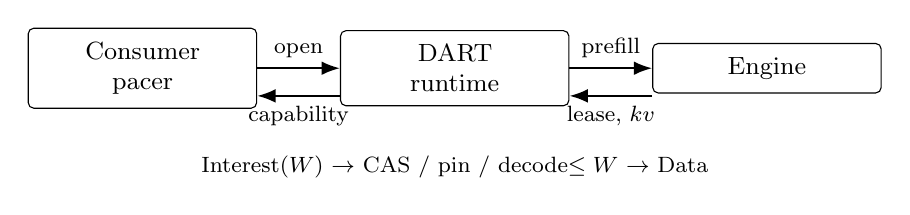
\begin{tikzpicture}[
  font=\small,
  box/.style={draw, rounded corners=2pt, align=center, inner sep=5pt, text width=2.55cm},
  arr/.style={-{Latex}, thick}
]
\node[box] (c) {Consumer\\pacer};
\node[box, right=1.05cm of c] (r) {DART\\runtime};
\node[box, right=1.05cm of r] (e) {Engine};
\draw[arr] (c) -- node[above,font=\footnotesize] {open} (r);
\draw[arr] (r) -- node[above,font=\footnotesize] {prefill} (e);
\draw[arr] ([yshift=-10pt]e.west) -- node[below,font=\footnotesize] {lease, $kv$} ([yshift=-10pt]r.east);
\draw[arr] ([yshift=-10pt]r.west) -- node[below,font=\footnotesize] {capability} ([yshift=-10pt]c.east);
\node[font=\footnotesize, below=0.5cm of r] (i) {Interest$(W)$ $\rightarrow$ CAS / pin / decode$\le W$ $\rightarrow$ Data};
\end{tikzpicture}
\caption{Prefill once. Subsequent work is credited Interests against a named continuation. Disconnect zeroes credit.}
\label{fig:loop}
\end{figure}

Figure~\ref{fig:loop} is the implemented loop.
Figure~\ref{fig:cake} is what DART owns versus what it reuses.

\begin{figure}[t]
\centering
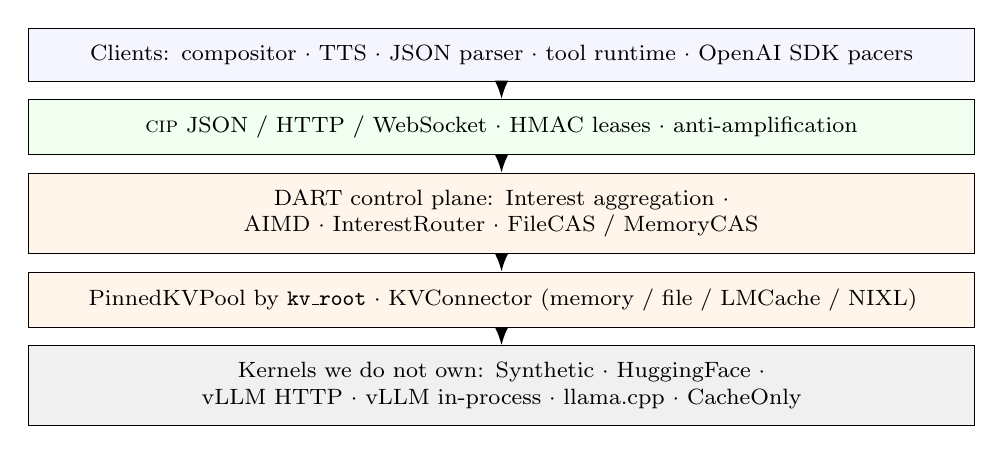
\begin{tikzpicture}[
  font=\footnotesize,
  layer/.style={draw, align=center, inner sep=6pt, text width=11.6cm},
  arr/.style={-{Latex}, thick}
]
\node[layer, fill=blue!4] (cli) {Clients: compositor $\cdot$ TTS $\cdot$ JSON parser $\cdot$ tool runtime $\cdot$ OpenAI SDK pacers};
\node[layer, fill=green!6, below=0.22cm of cli] (cip) {\cip{} JSON / HTTP / WebSocket $\cdot$ HMAC leases $\cdot$ anti-amplification};
\node[layer, fill=orange!8, below=0.22cm of cip] (rt) {DART control plane: Interest aggregation $\cdot$ AIMD $\cdot$ InterestRouter $\cdot$ FileCAS / MemoryCAS};
\node[layer, fill=orange!8, below=0.22cm of rt] (kv) {PinnedKVPool by \kvroot{} $\cdot$ KVConnector (memory / file / LMCache / NIXL)};
\node[layer, fill=gray!12, below=0.22cm of kv] (eng) {Kernels we do not own: Synthetic $\cdot$ HuggingFace $\cdot$ vLLM HTTP $\cdot$ vLLM in-process $\cdot$ llama.cpp $\cdot$ CacheOnly};
\draw[arr] (cli) -- (cip);
\draw[arr] (cip) -- (rt);
\draw[arr] (rt) -- (kv);
\draw[arr] (kv) -- (eng);
\end{tikzpicture}
\caption{Layer cake. Green/orange is the control plane. Grey is the residual stream. DART never ships a CUDA kernel.}
\label{fig:cake}
\end{figure}

\subsection{Runtime}

\texttt{DartRuntime} is one asyncio scheduler, one producer, in-process CAS by default.
\texttt{open} prefills, signs a lease, pins the initial \kvroot{}, and returns a handle.
The scheduler loop (Algorithm~\ref{alg:tick}) ticks on Interest wakeup or \texttt{poll\_interval}.

\begin{algorithm}[t]
\caption{SchedulerTick: skip when $W{=}0$; decode at most granted credits.}
\label{alg:tick}
\begin{algorithmic}[1]
\For{each live continuation $C$}
  \If{$C$ stopped or over quota}
    \State finish; Nack(\texttt{done}); \textbf{continue}
  \EndIf
  \If{lifetime expired and credits $>0$ and no waiter}
    \State timeout; discard draft
  \EndIf
  \If{credits $>0$ or grammar or pending Interest}
    \State wake KV / pin; add $C$ to ready
  \Else
    \State $\mathrm{skipped}{+}{+}$; pause(\texttt{keep}) or sleep pin; do not call decode
  \EndIf
\EndFor
\State batch $\gets$ ready$[:\texttt{max\_num\_seqs}]$
\For{$C$ in batch}
  \State $(n, K_{\mathrm{extra}}) \gets \mathrm{takeDecode}(\min(\mathrm{segment}, \mathrm{remaining}))$
  \State count $K_{\mathrm{extra}}$ as drafted; call $\mathrm{engine.decode}(C, n)$ only
  \State commit tokens; CAS.put(name); publish new \kvroot{}; complete waiters
\EndFor
\end{algorithmic}
\end{algorithm}

\texttt{consume} is the SDK helper: the pacer's \texttt{next\_window} becomes $W$, names advance with the child root, and \texttt{EXPIRED} retries (cap 8) so a slow engine is not a hard stop.
Grammar pacers name \texttt{grammar/span/next-value} instead of a token segment.

\subsection{Pin, connector, mesh}
\label{sec:mesh}

\texttt{PinnedKVPool} indexes engine state by \kvroot{}: token ids, sampler, extents, pos, segment index, holder, pin lease.
Sleep sets \texttt{on\_gpu=false} and does not drop the record.
Expiry drops it.
Eviction prefers sleeping, then oldest \texttt{last\_access}, and never the newest pin.
\texttt{adopt} transfers the holder and increments \texttt{prefills\_skipped} on the destination runtime: resume is installing named KV, not thawing a process.

Connectors expose \texttt{put}/\texttt{get}/\texttt{transfer}:

\begin{center}
\small
\begin{tabular}{lcc}
\toprule
Kind & Persistence & RDMA required \\
\midrule
\texttt{memory} & process & no \\
\texttt{file} & directory of JSON blobs & no \\
\texttt{lmcache} & same API; real library if installed & no for tests \\
\texttt{nixl} & accounts bytes/hops; \texttt{nixl-rdma} if importable else memcpy & no for tests \\
\bottomrule
\end{tabular}
\end{center}

A connector miss is a miss.
Decode already succeeded if \texttt{put} fails; the runtime logs and continues.
Handover without a blob is Nack \texttt{unknown\_name}, never a silent re-prefill.

\texttt{InterestRouter} (Algorithm~\ref{alg:route}) is not sticky to the prefill machine.
Cheapest is $\mathrm{cost}\times(1+\mathrm{awake\ seqs}) + \mathrm{gpu\_bytes}/10^9$.
A pin holder is preferred even when it is expensive: moving KV to a cheaper GPU is a handover, not the default.
Per-\kvroot{} asyncio lock: two concurrent Interests cannot split-brain adopt.

Handover steps: (1)~\texttt{release\_for\_handover} on the old node (pending Interests Nack \texttt{busy}; CAS still answers); (2)~\texttt{transfer} named KV (NIXL-shaped); (3)~dest \texttt{adopt}; (4)~dest satisfies the Interest.
\texttt{dart mesh --nodes 3} is the local form.

\begin{algorithm}[t]
\caption{RouteInterest($I$): CAS, then pin holder, then cheapest plus handover.}
\label{alg:route}
\begin{algorithmic}[1]
\State verify lease; lock on $I$'s \kvroot{}
\If{CAS has $I.n$}
  \State \Return Data, kind=\texttt{cas}
\EndIf
\If{a live node holds the pin}
  \State \Return that node's \textsc{HandleInterest}, kind=\texttt{pin}
\EndIf
\If{a live continuation matches $(\mathrm{cont\_id}, \kvroot{})$}
  \State \Return that node, kind=\texttt{local}
\EndIf
\State $d \gets$ cheapest node; pull KV blob; $d.\mathrm{adopt}$; decode
\State \Return Data, kind=\texttt{handover}, \texttt{prefill\_skipped}
\end{algorithmic}
\end{algorithm}

\subsection{Engines}
\label{sec:engines}

DART never owns the residual stream.
Table~\ref{tab:engines} is the adapter set.

\begin{table}[t]
\centering
\small
\caption{Engine adapters. Paper tables use the \emph{engine} kernel-launch counter, not only wrapper ticks.}
\label{tab:engines}
\begin{tabular}{llp{0.46\linewidth}}
\toprule
Flag & Class & Role \\
\midrule
\texttt{synthetic} & \texttt{SyntheticEngine} & Hash tokens, real extents; kill-test default \\
\texttt{hf} & \texttt{HuggingFaceEngine} & In-process weights; demo SmolLM2-135M \\
\texttt{vllm} & \texttt{VLLMChatEngine} & HTTP; each Interest is \texttt{max\_tokens}{=}$W$ \\
\texttt{vllm-inprocess} & \texttt{InProcessVLLMEngine} & Admit once; \texttt{waiting} + pinned blocks \\
\texttt{llamacpp} & \texttt{LlamaCppEngine} & HTTP \texttt{n\_predict}{=}$W$, \texttt{cache\_prompt} \\
\texttt{cache} & \texttt{CacheOnlyEngine} & FileCAS peer; never decodes \\
\bottomrule
\end{tabular}
\end{table}

HTTP adapters implement the \idd{} invariant without forking vLLM: they simply do not POST when $W{=}0$.
They re-enter the engine's request admission path on every credited Interest (Section~\ref{sec:limits}).
The in-process plugin is the tighter binding: \texttt{CreditGatedScheduler} admits once, pins blocks, and \texttt{schedule\_decode}($n$) moves \texttt{waiting} $\to$ \texttt{running} $\to$ \texttt{waiting}.
Memory pressure may evict unpinned prefix-cache victims, never a waiting pin.
\texttt{DART\_VLLM\_INPROCESS=1} plus the \texttt{vllm} package binds that scheduler to a live GPU process; tests use the synthetic residual stream in the same slots.

The kill-test measures the engine's \texttt{kernel\_launched} flag.
Empty output with that flag false is required when $n \le 0$.

\subsection{Implementation notes}

The repository is a Python 3.11 package (\texttt{src/dart/}): \texttt{core} (runtime, leases, CC), \texttt{cip} (names, Merkle), \texttt{kv} (CAS, pin, connectors), \texttt{mesh}, \texttt{engine}, \texttt{api} (FastAPI + demo compositor), \texttt{client} (SDK, pacers), \texttt{eval} (paper suite).
Public imports stay stable: \texttt{from dart import DartRuntime, Interest, ReadingPacer}.
Metrics: Prometheus \texttt{/metrics} and JSON \texttt{/v1/metrics}, including \texttt{dart\_decode\_steps\_skipped}, pin adopts, and engine launches.
\texttt{GET /v1/engine} compares local HTTP POSTs with the engine process forward counter.

\FloatBarrier
\section{Evaluation}
\label{sec:eval}

All numbers in this section are from \texttt{dart experiment --suite paper} (\texttt{--seconds 1.0 --max-tokens 96}) unless noted.
The producer is \texttt{SyntheticEngine} (eight layers, GQA-shaped extents, 32\,KiB per layer-block, hash-based tokens).
That is a control-plane measurement with real KV accounting, not a GPU-fleet result.
Paper tables report \emph{engine} kernel launches (successful generate/completion), not only wrapper ticks.
Prompt is fixed: ``Write a long essay about named continuations.''

Survive (kill-test): generated $< 0.9\times$ push or lower KV high-water, with consumption $> 0$.

\subsection{Kill test: push versus credit}
\label{sec:kill}

\begin{table}[t]
\centering
\small
\caption{Push drain versus credit-gated pacers. Unconsumed is generated minus consumed. KV high-water is named extent bytes. Skipped ticks are scheduler loops with $W{=}0$.}
\label{tab:kill}
\begin{tabular}{lrrrrr}
\toprule
Arm & Gen. & Cons. & Eng.\ launches & Skipped & KV HW \\
\midrule
Push (drain) & 96 & 96 & 6 & 0 & 1.75\,MiB \\
IDD 30\,tok/s & 46 & 46 & 31 & 90 & 1.00\,MiB \\
API 200\,tok/s & 96 & 96 & 81 & 32 & 1.75\,MiB \\
JSON bursty & 21 & 21 & 21 & 93 & 0.75\,MiB \\
\bottomrule
\end{tabular}
\end{table}

Table~\ref{tab:kill} is the inversion test.

Push uses \texttt{DrainPacer} with a large window: the kernel runs until the 96-token cap.
Six launches of 16-token segments fill the quota.
KV high-water is 1\,835\,008\,B ($1.75$\,MiB): prompt plus 96 outputs span seven 16-token blocks times eight layers times 32\,KiB.

IDD at 30\,tok/s generates 46 tokens and consumes 46.
Unconsumed is 0.
Generated-token cut versus push is $50/96 = 52\%$.
KV high-water cut is $(1.75-1.00)/1.75 = 43\%$ (four blocks instead of seven).
It launches \emph{more} kernels (31 vs.\ 6) because each Interest is a short $W$, not one long push.
The engine still only runs when credited; launch count is not the objective.
Ninety scheduler ticks skip decode.
The kill test survives.

API at 200\,tok/s can absorb the cap in one second, so generated tokens match push.
Launches rise (81) because the pacer still segments.
Skipped ticks drop to 32.
This arm exists to show that \idd{} is not ``always generate less'': if the consumer can take 96 tokens, the producer may emit 96.
The gate follows demand.

JSON bursty (\texttt{JsonNeedPacer}, burst 64, pause 50\,ms) generates 21 tokens, 21 launches, 93 skips, 0.75\,MiB KV.
A parser that pauses between values should not pay for an essay.

\subsection{Andes-complete}
\label{sec:andes}

\begin{table}[t]
\centering
\small
\caption{Andes watermark pause versus IDD refuse-to-decode. Capture is Andes' generated-token win over push divided by IDD's. Kill if capture $\ge 90\%$ and Andes inventory stays at the watermark.}
\label{tab:andes}
\begin{tabular}{lrrrr}
\toprule
Arm & Generated & Eng.\ launches & Inventory HW & Capture of IDD \\
\midrule
Push & 96 & 6 & 0 & --- \\
Andes ($W{=}32$) & 62 & 32 & 32 & 0.68 \\
IDD 30\,tok/s & 46 & 31 & 0 & 1.00 \\
\bottomrule
\end{tabular}
\end{table}

Andes is reimplemented against the same synthetic producer: generate into a buffer, pause while $\lvert \mathrm{buffer} \rvert \ge 32$, consume at 30\,tok/s.
It generates 62 tokens (35\% cut vs.\ push) and holds 32 unread tokens at high-water.
Once the buffer sits at the watermark, further launches are 1-token top-ups as the consumer drains---hence 32 engine launches, not four large chunks.

IDD generates 46 (52\% cut vs.\ push, 26\% cut vs.\ Andes).
Inventory high-water is 0: there is no unread buffer, because those tokens were not encoded.

Andes' win over push is $96-62=34$ tokens.
IDD's win is $96-46=50$.
Capture is $34/50=0.68$.
The Andes-complete kill requires capture $\ge 0.90$ \emph{and} Andes inventory at the watermark.
The second clause is true; the first is not.
The kill does \emph{not} fire.
\cip{} is not an Andes patch.

The qualitative tell is inventory, not the 16-token gap alone.
Andes can be tuned (smaller watermark, slower consume) to generate less.
It cannot make unread inventory zero without refusing to decode---at which point it has become \idd{}.

\subsection{Grammar jump-forward}
\label{sec:grammar}

\begin{table}[t]
\centering
\small
\caption{Typed Interest for \texttt{grammar/span/tool-args}. Jump-forward emits one named Data. Logit masking pays one kernel per constrained token.}
\label{tab:grammar}
\begin{tabular}{lrrr}
\toprule
Arm & Kernel launches & Tokens (ids) & Text bytes \\
\midrule
Logit masking & 36 & 36 & 36 \\
Jump-forward & 1 & 3 & 36 \\
\bottomrule
\end{tabular}
\end{table}

Table~\ref{tab:grammar}: the span \texttt{\{"name":"search","query":"dart idd"\}} is one Interest.
Jump-forward tokenizes it as three ids in one kernel and stores one Data.
Masking walks the span a token at a time: 36 launches, ratio 36.
SGLang/XGrammar already jump inside one process~\citep{zheng2024sglang,dong2024xgrammar}.
The DART claim is the name: a peer can satisfy the same span from CAS.

\subsection{CAS peer}
\label{sec:cas}

Process A decodes into \texttt{FileCAS}.
Process B starts with \texttt{CacheOnlyEngine} on the same directory and \texttt{satisfy\_named} the CIP name.

Result: \texttt{peer\_cache\_hit=true}, producer launches $=1$, peer launches $=0$, texts match, \texttt{peer\_gpu=false}.

That is the not-Andes defense.
The continuation object is the cache unit.
A GPU-less peer is a valid producer for a name that already exists.
Per-token HTTP replay cannot do this without re-running the kernel or sharing a process.

\subsection{Mesh handover}
\label{sec:mesheval}

Three in-process nodes, NIXL-shaped connector, costs $(10, 5, 1)$ so node-2 is cheapest.
Open on node-0 (one prefill).
Table~\ref{tab:mesh} is the route vector.

\begin{table}[t]
\centering
\small
\caption{Three-node mesh. Kernel vector is $(\mathrm{node\textrm{-}0}, \mathrm{node\textrm{-}1}, \mathrm{node\textrm{-}2})$. Prefills stay $(1,0,0)$ after handover: node-2 adopted.}
\label{tab:mesh}
\begin{tabular}{llrrl}
\toprule
Step & Kind & Node & Kernels after & Note \\
\midrule
Interest seg/0 & pin & node-0 & $(1,0,0)$ & first decode on holder \\
Repeat name & cas & CAS & $(1,0,0)$ & no extra kernel \\
Interest seg/1 & pin & node-0 & $(2,0,0)$ & holder beats cheaper node-2 \\
After release, seg/2 & handover & node-2 & $(2,0,1)$ & 512\,KiB transfer, skip prefill \\
\bottomrule
\end{tabular}
\end{table}

Assertions that all hold: CAS text equals the first Data; pin route stays on node-0 even though node-2's score is lower; handover reports \texttt{prefill\_skipped}, \texttt{transfer\_bytes}{=}$524288$, destination \texttt{prefills}{=}0, and a positive token count.
Changing machines did not live-migrate a request.

\subsection{Waiting plugin versus HTTP admission}

Idle $W{=}0$ after \texttt{open}: 1 admission, 1 prefill forward, 0 decode forwards, 1 request in \texttt{waiting}, 8 pinned blocks (256\,KiB), 0 evictions.

Two Interests: 2 decode forwards, still 1 admission, 0 re-entries, still 8 pinned blocks, request returns to \texttt{waiting}.

Memory pressure: an unpinned prefix-cache victim (4 blocks) is evicted; the waiting pin survives.

HTTP fake-vLLM on the same two Interests: 2 generate POSTs (admission twice).

The plugin tightens KV residency and admission.
It does not invent credit-gated decode---the HTTP path already refused to POST at $W{=}0$.
It avoids the re-entry the HTTP path still pays.

\section{Discussion}
\label{sec:disc}

\paragraph{Control plane versus kitchen.}
A GPU fleet is the kitchen: occupancy batching, paged KV, disaggregation, RDMA.
DART is the waiter: it will not send food the table has not ordered.
Building a waiter is not building a kitchen, and measuring the waiter on a synthetic producer is not a cluster tok/s number.
The paper suite is designed so a reviewer can rerun \texttt{dart experiment --suite paper} and get the same cuts.

\paragraph{More launches, less work.}
IDD 30\,tok/s launches 31 kernels versus push's 6.
That is expected.
Each kernel is a short credited window.
The objective is generated tokens, unread inventory, and KV high-water---not launch count.
A production in-process plugin can coalesce ready continuations into one batched forward; HTTP adapters cannot without re-entering admission.

\paragraph{Demand following.}
API 200\,tok/s matches push on tokens.
JSON bursty does not.
The same invariant covers both: follow $W$, do not invent a second policy for ``fast clients.''

\paragraph{Why names.}
Pin and CAS are not optional decorations on a credit gate.
Without names, a second process cannot answer, handover is live-migration, and grammar jump is trapped in one engine.
The Merkle root is deliberately not a proof; it is a lookup key.

\paragraph{Fill-from-other-demand.}
If a packed cluster idles SM cycles because the credit-ready set is small, those cycles should go to prefill, embeddings, or offline batch---not to unread decode.
We do not measure tok/J here (criterion~2).
Declaring energy victory from Table~\ref{tab:kill} would be a category error.

\section{Limitations}
\label{sec:limits}

DART is not a finished GPU fleet that replaces vLLM.
HTTP \texttt{VLLMChatEngine} / \texttt{LlamaCppEngine} re-enter admission; a load spike can 503 a live continuation; prefix cache may evict and force re-prefill.
\idd{} still did not decode without credit; it may pay a re-prefill pinned blocks would have avoided.
Measure \texttt{GET /v1/engine}: local POSTs versus the engine process forward counter.

Real NIXL RDMA and LMCache GPU pages are optional.
Tests use memcpy.
Metrics report \texttt{rdma\_available=false} when the library is absent.
\texttt{CreditGatedScheduler} binds to a live GPU vLLM process only when the \texttt{vllm} package is present and \texttt{DART\_VLLM\_INPROCESS=1}.
The waiting-plugin numbers in Section~\ref{sec:eval} use the in-process synthetic residual stream.

The Hugging Face path (SmolLM2-135M-Instruct) is a real-model demo of the same CIP, not the paper-suite producer.
We do not mix those numbers into Tables~\ref{tab:kill}--\ref{tab:mesh}.

Speculative $K$ is a signal.
Uncredited draft is not executed.
A producer with verified rollback is future kernel work, not a hidden flag.

If credit gating dropped consumed tok/J because the GPU went idle, fill-from-other-demand must be enabled before declaring death (criterion~2).
Per-token names are forbidden; segments stay 8--32 tokens (criterion~3).

We do not claim an IETF standard, an NDN deployment, or MOQ interoperability.

\section{Conclusion}
\label{sec:conc}

Serving should not encode segments nobody has credit to consume.
DART makes that a protocol: named continuations, token windows, CAS then pin then decode, handover as the next Interest from a new locator.
The kernels stay the kernels.
The scheduler is a congestion controller.
The paper suite is in the repository; the Andes-complete kill did not fire; the HTTP honesty clause remains.

{\small
\bibliographystyle{unsrtnat}
\bibliography{references}
}

\appendix
\section{Paper-suite command}
\label{app:cmd}

\begin{verbatim}
dart experiment --suite paper --seconds 1.0 --max-tokens 96
\end{verbatim}

Arms: push drain, reading 30\,tok/s, API 200\,tok/s, JSON bursty, Andes watermark 32, grammar \texttt{tool-args}, FileCAS peer, three-node NIXL-shaped mesh, waiting plugin versus HTTP fake-vLLM.
Default synthetic seed is 0 for kill/Andes, 1 for grammar, 3 for CAS, 11 for mesh, 2 for waiting.
Install the package in editable mode, then rerun from the repository root.

\section{Default configuration}
\label{app:cfg}

Paper runs use \texttt{RuntimeConfig} with \texttt{segment\_size}{=}16, \texttt{w\_init}{=}16 (128 for push), \texttt{w\_max}{=}128 (512 for push), \texttt{startup\_credit}{=}16, \texttt{poll\_interval\_s}{=}0.002, \texttt{interest\_lifetime\_s}{=}5, \texttt{lease\_ttl\_s} $\ge 60$.
Synthetic \texttt{ModelConfig}: 8 layers, 8 KV heads, head dim 64, block size 16, f16, vocab 32\,000.
Extent bytes $= 2 \times 8 \times 64 \times 16 \times 2 = 32$\,KiB; KV high-water scales with occupied blocks times layers.

\section{Module map}
\label{app:mod}

\texttt{dart.core.runtime} scheduler and Interest handler;
\texttt{dart.core.cc} AIMD;
\texttt{dart.core.lease} HMAC capability;
\texttt{dart.cip.protocol} names and messages;
\texttt{dart.cip.merkle} \kvroot{};
\texttt{dart.kv.pin} pin table;
\texttt{dart.kv.kvconn} connectors;
\texttt{dart.mesh.router} CAS/pin/handover;
\texttt{dart.engine.*} adapters;
\texttt{dart.eval.experiment} \texttt{paper\_suite};
\texttt{dart.client.consumers} pacers.
Kill criteria and HTTP honesty: repository \texttt{docs/limitations.md}.

\end{document}
